\documentclass[10pt]{article}
\usepackage{icmlko}

\icmlmeta{IP 파운데이션 월드모델}{22}{어디에 투자할 것인가}{표본은 200건에서 수익이 끝나고 미디어 투입은 빼는 편이 낫다 --- 값진 것은 매장 노출도다}

\begin{document}

\twocolumn[
\icmlheader

\begin{abstract}
스물한 편이 방법을 세웠다. 이 노트는 자원 배분을 묻는다 --- 다음 노력을 어디에
쓸 것인가. 세 가지를 쟀다. 첫째, 노트 21이 남긴 실무 조건 검정 ---
무작위 k건이 아니라 \textbf{먼저 열린 k건}으로 눈금을 잡으면 어떻게 되는가.
팝업은 오히려 낫고(2.52--2.87배 대 무작위 2.67--3.25배), 아이돌은 k=5에서
파탄했다가(8.39배) k$\geq$8부터 회복해 상수를 이긴다. \textbf{초기 몇 건만으로
눈금을 잡는 것은 위험하다.} 둘째, 출처 표본을 늘리면 얼마나 좋아지는가 ---
게임을 50건에서 482건까지 늘리며 재니 \textbf{200건에서 포화한다}. 200건에서
게임 $\to$ 팝업 $-$0.0886, 482건에서 $-$0.0671로 오히려 줄어든다. 셋째, 축의
값어치 --- 팝업에서 하나씩 빼 보니 \textbf{매장 노출도가 가장 값지고}(제거 시
전이가 $-$0.0718에서 $-$0.0408로 43\% 악화) \textbf{미디어 투입은 빼는 편이
낫다}(제거 시 $-$0.0816으로 개선). 노트 20이 게임에서 발견한 미디어 투입의
문제가 팝업에서도 확인된다. 투자 우선순위가 나온다 --- 매장 노출도를 다른
도메인에서 관측 가능하게 만드는 것이 첫째, 미디어 투입 폐기가 둘째, 표본 확대는
셋째다.
\end{abstract}
]

\section{실무 조건에서 다시 잰다}

노트 21은 눈금 보정에 필요한 라벨 수를 쟀는데, k개를 \emph{무작위}로 뽑았다.
같은 노트의 한계 절에 이렇게 적었다.

\begin{quote}\fontsize{9.2}{11}\selectfont
k개 라벨은 무작위 추출을 가정한다. 실무에서는 먼저 열리는 것부터 실측하므로
시간 순서가 섞인다.
\end{quote}

먼저 열린 k건으로 눈금을 잡고 나머지에서 검정했다.

\begin{figure}[t]
\centering
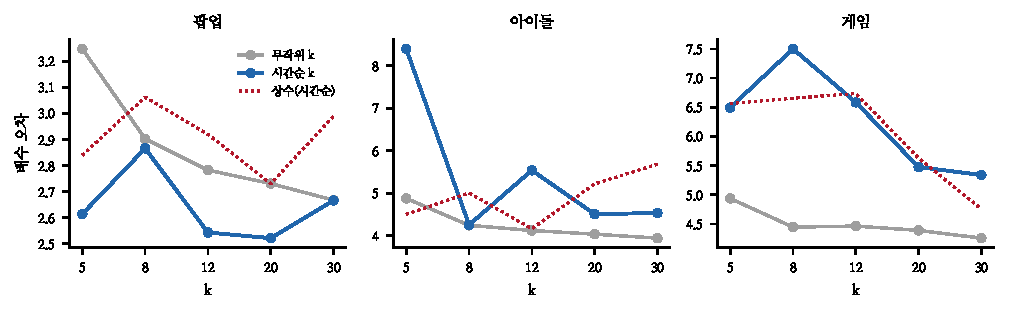
\includegraphics[width=\textwidth]{figs/time.pdf}
\caption{무작위 k건과 시간순 k건의 비교. 도메인마다 다르다.}
\end{figure}

\begin{table}[t]
\centering\tsize
\caption{눈금 보정 방식별 배수 오차.}
\begin{tabular}{lrrrr}
\toprule
도메인 & k & 무작위 & 시간순 & 상수(시간순) \\
\midrule
팝업 & 5 & 3.25 & \textbf{2.61} & 2.84 \\
팝업 & 12 & 2.78 & \textbf{2.54} & 2.92 \\
팝업 & 20 & 2.73 & \textbf{2.52} & 2.73 \\
\midrule
아이돌 & 5 & 4.88 & \textbf{8.39} & 4.50 \\
아이돌 & 8 & 4.24 & 4.26 & 5.01 \\
아이돌 & 20 & 4.04 & 4.51 & 5.22 \\
\midrule
게임 & 8 & 4.44 & 7.50 & 6.66 \\
게임 & 30 & 4.26 & 5.34 & 4.75 \\
\bottomrule
\end{tabular}
\end{table}

팝업은 시간순이 \emph{더 낫다}. 초기 표본이 전체를 잘 대표했다는 뜻이다.

아이돌은 k=5에서 8.39배로 파탄한다. 무작위 5건의 4.88배와 비교하면 두 배 가까이
나쁘다. 원인은 표본 구성이다 --- 아이돌 표본은 2013년부터 2026년까지인데 초기
데뷔의 초동이 훨씬 작았다. 그 다섯 건으로 눈금을 잡으면 전체를 크게 과소평가한다.
k=8부터 회복되고, 그 뒤로는 시간순 상수를 계속 이긴다(4.26 대 5.01, 4.51 대 5.22).

\claimx{시간이 흐르며 반응 규모가 커진 도메인에서는 먼저 열린 소수로 눈금을 잡으면
안 된다. 아이돌 k=5에서 배수 오차가 무작위의 1.7배로 뛴다. 여덟 건부터 안정된다.}{탈추세를
더 정교하게(2차 이상, 구조 변화 반영) 하면 k=5에서도 안정되는 경우, 문제는 표본
구성이 아니라 추세 모형이었다.}

\section{표본은 200건에서 포화한다}

출처 도메인의 표본을 늘리면 계수 추정이 정밀해진다. 어디까지 유효한가.
게임을 50건에서 482건까지 부분표집하며 전이를 쟀다.

\begin{figure}[t]
\centering

\includegraphics[width=\columnwidth]{figs/curve.pdf}
\caption{출처 표본 크기와 전이 강도. 빈 원은 유의하지 않은 점이다.}
\end{figure}

\begin{table}[t]
\centering\tsize
\caption{게임을 출처로 쓸 때 표본 크기의 효과.}
\begin{tabular}{rrrrr}
\toprule
& \multicolumn{2}{c}{게임 $\to$ 팝업} & \multicolumn{2}{c}{게임 $\to$ 아이돌} \\
게임 n & 차이 & p & 차이 & p \\
\midrule
50 & $-$0.0912 & 0.025 & $-$0.0481 & 0.107 \\
100 & $+$0.0294 & 0.639 & $-$0.0123 & 0.299 \\
\textbf{200} & \textbf{$-$0.0886} & \textbf{0.000} & \textbf{$-$0.0814} & \textbf{0.000} \\
300 & $-$0.0725 & 0.001 & $-$0.0791 & 0.000 \\
482 & $-$0.0671 & 0.001 & $-$0.0752 & 0.000 \\
\bottomrule
\end{tabular}
\end{table}

200건에서 최대치이고, 그 뒤로는 오히려 조금 줄어든다. 100건에서 나온 이상치
($+$0.0294)는 그 부분표본의 인자 구조가 불안정했던 것으로 보인다 --- 50건과
200건이 모두 음수인데 100건만 양수다.

\claimx{출처 표본을 늘리는 이득은 200건 부근에서 끝난다. 482건은 200건보다 낫지
않다.}{다른 출처 도메인에서도 200건 부근에서 포화하면 일반 규칙이고, 도메인마다
포화점이 다르면 이것은 게임 표본의 성질이다.}

이것은 자원 배분에 직접 쓰인다. 새 도메인을 열 때 200건을 목표로 하고, 그 이상은
다른 곳에 쓴다.

\section{축마다 값어치가 다르다 --- 하나는 음수다}

팝업은 다섯 축을 모두 관측한다. 하나씩 빼고 전이를 재면 그 축의 값어치가 나온다.
공통 축인 타깃 폭과 굿즈 규모는 정렬에 필요하므로 뺄 수 없고, 나머지 셋을 뺐다.

\begin{figure}[t]
\centering
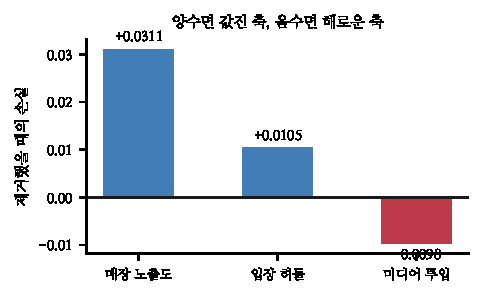
\includegraphics[width=\columnwidth]{figs/axis.pdf}
\caption{축을 제거했을 때의 손실. 양수면 값진 축, 음수면 해로운 축이다.}
\end{figure}

\begin{table}[t]
\centering\tsize
\caption{팝업에서 축 하나를 제거했을 때. 대상은 팝업, 출처는 나머지 둘의 평균.}
\begin{tabular}{lrr}
\toprule
구성 & 전이 차이 & 손실 \\
\midrule
전부 사용 & $-$0.0718 & --- \\
\midrule
매장 노출도 제거 & $-$0.0408 & \textbf{$+$0.0311} \\
입장 허들 제거 & $-$0.0614 & $+$0.0105 \\
미디어 투입 제거 & $-$0.0816 & \textbf{$-$0.0098} \\
\bottomrule
\end{tabular}
\end{table}

\paragraph{매장 노출도가 가장 값지다}
빼면 전이가 43\% 악화된다. 그런데 이 축은 아이돌에서 32\%, 게임에서 0\%다.
\emph{가장 값진 축이 가장 안 재진다.}

\paragraph{미디어 투입은 빼는 편이 낫다}
제거하면 오히려 좋아진다($-$0.0718 $\to$ $-$0.0816). 노트 20은 게임에서 미디어
투입을 추가했다가 전이가 나빠져 되돌렸는데, 같은 문제가 팝업에서도 확인된다.
세 도메인에서 서로 다른 물리량을 재는 축이므로 어느 도메인에 있든 인자 공간을
왜곡한다.

\claimx{미디어 투입 축은 현재 정의로는 해롭다. 게임에서 추가하면 전이가 나빠지고
(노트 20) 팝업에서 제거하면 좋아진다. 정의를 통일하기 전까지 이 축은 쓰지 않는다.}{세
도메인에서 같은 물리량으로 재정의한 뒤 제거 손실이 양수로 돌아서면, 축은 옳고
측정만 어긋났던 것이다.}

\section{그래서 투자 우선순위}

\begin{enumerate}[leftmargin=1.3em,itemsep=0.25em]
\item \textbf{매장 노출도를 다른 도메인에서 관측 가능하게 만든다.} 가장 값진 축인데
      아이돌 32\%, 게임 0\%다. 이것 하나가 표본을 두 배 늘리는 것보다 낫다.
\item \textbf{미디어 투입을 폐기하거나 재정의한다.} 현재 정의로는 음의 값어치다.
\item \textbf{표본은 도메인당 200건까지만.} 그 이상은 수익이 없다.
\end{enumerate}

이 순서는 앞선 노트들과 정합한다. 노트 13은 공유 슬롯 수가 관측 가능성의 교집합에
갇힌다고 했고, 노트 18--19는 인자로 그 제약을 풀었지만 여전히 \emph{각 도메인이
무엇을 재는가}가 성능을 정한다. 재는 축을 늘리는 것이 표본을 늘리는 것보다
효율적인 이유다.

\section{한계}

\begin{itemize}[leftmargin=1.1em,itemsep=0.15em]
\item 축 절제는 팝업 하나에서만 했다. 다른 도메인은 관측 축이 둘에서 셋뿐이라
      뺄 것이 없다.
\item 표본 포화는 게임 한 도메인에서 관측했다. 100건의 이상치가 곡선 해석을
      흐린다.
\item 시간순 검정은 단일 분할이므로 반복 없이 한 번의 결과다. 무작위 쪽은
      200회 반복이라 비교가 비대칭이다.
\item ``매장 노출도가 값지다''는 팝업 기준이다. 다른 도메인에서 관측하게 만들었을 때
      같은 값어치일지는 모른다 --- 노트 20의 미디어 투입이 정확히 그렇게 실패했다.
\end{itemize}

\section{다음}

\begin{enumerate}[leftmargin=1.3em,itemsep=0.15em]
\item 매장 노출도의 도메인 독립 정의 --- ``그 대상이 닿기 쉬운 자리인가''를 세
      도메인에서 같은 물리량으로.
\item 시간순 검정을 여러 분할로 반복해 비교를 대칭으로.
\item 탈추세 모형 개선 --- 아이돌 k=5 파탄이 추세 모형 탓인지 확인.
\item 네 번째 도메인에서 포화점 재확인.
\end{enumerate}

\vspace{0.6em}
\hrule height 0.3pt
\vspace{0.5em}
{\footnotesize
\textbf{참고문헌}\\[0.3em]
Guyon, I., Elisseeff, A. (2003). An introduction to variable and feature selection.
\emph{JMLR}, 3, 1157--1182.\\[0.15em]
Meredith, W. (1993). Measurement invariance, factor analysis and factorial
invariance. \emph{Psychometrika}, 58(4), 525--543.\\[0.15em]
Riley, R. D. et al. (2019). Minimum sample size for developing a multivariable
prediction model. \emph{Statistics in Medicine}, 38(7), 1262--1275.\\[0.15em]
Ben-David, S. et al. (2010). A theory of learning from different domains.
\emph{Machine Learning}, 79(1--2), 151--175.
}

\end{document}
